Per manifattura additiva si intende un qualsiasi processo di costruzione di oggetti, o parti di oggetti, tridimensionali
attraverso il deposito di sottili strati di materia in maniera guidata digitalmente \cite{DebRoyT2018Amom}.
Questo tipo di manifattura permette di produrre parti estremamente complesse senza il bisogno di dover costruire
costose sagome o stampi per colature a caldo. Un'altro grande vantaggio è quello di poter realizzare parti in singoli blocchi,
senza la necessità di dover assemblare pezzi, fattore che implica una rigidità strutturale elevata in quanto eventuali giunti o fori sono assenti.
La mancanza di pezzi di assemblaggio rende anche meno costoso lo stoccaggio e la gestione di elementi, abbassando notevolmente il costo per prodotto.
I settori che stanno traendo beneficio da questo tipo di manifattura sono quelli aeresopaziali, medici, energetici e automobilistici.
Negli ultimi vent'anni la manifattura additiva ha raggiunto livelli di qualità critici, soprattutto grazie all'evoluzione
delle piattaforme di high-performance computing, dello stoccaggio e del trattamento dei materiali metallici, dell'efficienza raggiunta dai laser ad alta potenza
e dallo studio di leghe metalliche complesse.

Inizialmente la manifattura additiva è stata impiegata soprattutto nel campo della prototipazione di design,
componenti la cui funzionalità principale era quella di mostrare un concetto piuttosto che implementarlo.
La ricerca nei settori sopracitati ha portato alla sperimentazione e al successivo utilizzo di manifattura additiva con materiali metallici, 
proprio per l'abilità di creare strutture complesse senza assemblaggio e quindi pronte all'uso.
La produzione attraverso manifattura additiva metallica pone diversi problemi all'attenzione di chi la utilizza, in primis i problemi relativi all'utilizzo in ambienti ad alta temperatura
(come per esempio ugelli di motori a reazione).

Il campo della manifattura additiva è relativamente giovane ed è sicuramente ancora agli albori,
ma la necessità di creare strutture sempre più complesse, sia in termini di grandezza che in termini di forma, sta spingendo 
sempre di più la ricerca verso diverse forme e processi, oltre che verso lo studio di innovative leghe metalliche.
\begin{figure}[H]
    \centering
    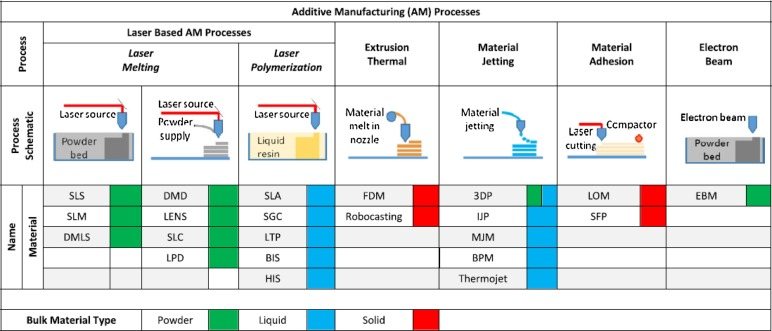
\includegraphics[width=\linewidth]{figure/ad.jpg}
    \caption{Vari processi di manifattura additiva.}
\end{figure}

\section{Processo LMD}
Esistono diversi processi per realizzare componenti attraverso la manifattura additiva,
questo progetto di tesi prende in evidenza un tipo particolare di processo chiamato Laser Metal Deposition.
I processi LMD sono un emergente categoria di processi di manifattura additiva che consistono nella creazione
di componenti metalliche dense attraverso l'applicazione di polveri metalliche stratificate, opportunamente fuse attraverso un raggio laser \cite{ZhangKai2014Coss}.
I macchinari che utilizzano questo processo utilizzano un raggio laser che crea un piccolo bacino di polvere fusa o sopra la superficie o sopra uno strato precedentemente fuso.
Il laser utilizzato viene regolato attraverso delle lenti focali per concentrarne il fascio alla distanza corretta.
Queste polveri sono veicolate sul substrato attraverso un ugello coassiale ebro di gas protettivi anti-ossidazione, per esempio azoto o argon.
Il flusso di gas all'interno dell'ugello è fondamentale poiché la scarsità di esso compromette la posa del materiale in quanto favorisce ossidazione, mentre l'abbondanza
aumenta la velocità del flusso e delle particelle spazzandole dalla superficie.
La riuscita di questo processo sta proprio nel calibrare correttamente il flusso del gas, la quantità di particelle immesse nell'ugello per unità di tempo e la potenza del laser.
Per coadiuvare il processo di posa dei materiali spesso si utilizzano degli ugelli capaci di regolare la distanza dalla superficie, i più avanzati inoltre regolano in maniera indipendente
angolo di posa e distanza su più assi. Poiché l'energia cinetica delle particelle in uscita dall'ugello è di gran lunga superiore alla forza di gravità si può anche pensare di depositare materiale 
con specifici bracci robotici capaci di variare la posizione e l'angolo dell'ugello su 5 o 6 assi, garantendo la costruzione di forme ancora più complesse attraverso la posa verticale dei materiali.

Le particelle solitamente variano in diametro fra 40\textmu\text{m} e 150\textmu\text{m}.
Il materiale usato può variare, vengono usate principalmente leghe d'acciaio, titanio o alluminio. 

\begin{figure}[H]
    \centering
    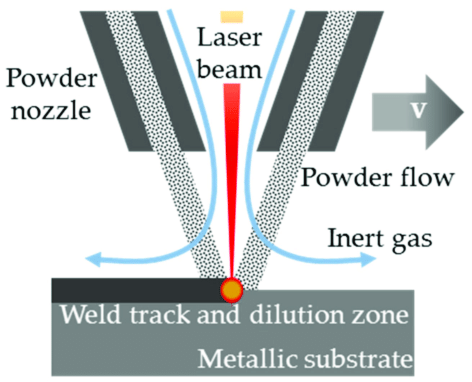
\includegraphics[width=\linewidth]{figure/lmd.png}
    \caption{Raffigurazione di un ugello LMD.}
\end{figure}

L'obiettivo principale di questa tesi consiste nel creare un applicativo in grado di simulare numericamente
scenari di Laser Metal Deposition da un punto di vista di emissione di particelle. In particolare durante lo sviluppo del solutore
sono stati concentrati gli sforzi sul simulare l'interazione tra le particelle di metallo e i seguenti componenti:
\begin{itemize}
    \item Pareti dei canali dell'ugello (analisi deviazione particelle)
    \item Flusso di gas
    \item Temperatura flusso
    \item Temperatura laser
\end{itemize}

